\documentclass{article}

% if you need to pass options to natbib, use, e.g.:
% \PassOptionsToPackage{numbers, compress}{natbib}
% before loading nips_2016
%
% to avoid loading the natbib package, add option nonatbib:
% \usepackage[nonatbib]{nips_2016}

%\usepackage{nips_2016}

% to compile a camera-ready version, add the [final] option, e.g.:
 \usepackage[final]{nips_2016}

\usepackage[utf8]{inputenc} % allow utf-8 input
\usepackage[T1]{fontenc}    % use 8-bit T1 fonts
\usepackage{hyperref}       % hyperlinks
\usepackage{url}            % simple URL typesetting
\usepackage{booktabs}       % professional-quality tables
\usepackage{amsfonts}       % blackboard math symbols
\usepackage{nicefrac}       % compact symbols for 1/2, etc.
\usepackage{microtype}      % microtypography
\usepackage{graphicx}

\title{Predicting Soccer Match Results With Bet Data}

% The \author macro works with any number of authors. There are two
% commands used to separate the names and addresses of multiple
% authors: \And and \AND.
%
% Using \And between authors leaves it to LaTeX to determine where to
% break the lines. Using \AND forces a line break at that point. So,
% if LaTeX puts 3 of 4 authors names on the first line, and the last
% on the second line, try using \AND instead of \And before the third
% author name.

\author{
	Zhenghan Zhang \\
	Harvey Mudd College\\
	Claremont, CA 91711 \\
	\texttt{zzhang@g.hmc.edu} \\
	%% examples of more authors
	 \And
	 Zhepei Wang \\
	 Harvey Mudd College \\
	 Claremont, CA 91711 \\
	 \texttt{zhwang@g.hmc.edu} \\
	%% \And
	%% Coauthor \\
	%% Affiliation \\
	%% Address \\
	%% \texttt{email} \\
}

\begin{document}
	% \nipsfinalcopy is no longer used
	
	\maketitle
	\begin{abstract}
		This paper presents a few algorithms to predict the result of a soccer match given a set of three gambling odds. The algorithms include a polynomial regression algorithm, a classification algorithm on an integrated feature, and a support vector machine algorithm on multiple features. We analyzed the accuracy and efficiency of these algorithms based on a dataset over 100,000 matches over the past 20 years.
%		The abstract paragraph should be indented \nicefrac{1}{2}~inch
%		(3~picas) on both the left- and right-hand margins. Use 10~point
%		type, with a vertical spacing (leading) of 11~points.  The word
%		\textbf{Abstract} must be centered, bold, and in point size 12. Two
%		line spaces precede the abstract. The abstract must be limited to
%		one paragraph.
	\end{abstract}
	
	\section{Introduction}
	There are millions of soccer fans around the world who are enthusiastic about predicting the results of soccer games. In particular, many soccer fans rely heavily on the odds handicap provided by gambling bet companies. However, gamblers normally will just analyze the odds data of one upcoming game and try to make their best bet out of it. After learning different methods of analyzing big data, we are curious whether gamblers could make a even better bet by using odds data and results of all previous soccer games.
	
	We obtained a wide range of odds data for games from \url{http://football-data.co.uk/data.php}. These data include the full-time scores for each individual match, and the odds handicap from over 10 gambling bet companies. There are roughly 400 matches for each season and each league, and the data set includes data for over 15 seasons. We have data from 4 leagues from England, 3 leagues from Scotland, 2 leagues from Germany, 2 leagues from Spain, 2 leagues from Italy, 2 leagues from France, and 1 league from Portugal. The range of data, which covers most of the major soccer leagues in Europe and different divisions for each country, will help us eliminate compound variables  as much as possible. Nine-tenth of the dataset will be used as training data, while the rest tenth will be the validation data.
	
	Before discussing the fitting algorithms,we first described a model to process the bet data and the score data. Then, to investigate the relationship between the match results and the betting odds data, we first did a naive algorithm, choosing the minimum of the betting odds to be the prediction. Then, we tried a polynomial regression model, a multi-class classification algorithm with a single, integrated feature, and a support vector machine algorithm. The naive algorithm, without training any data, has a poor performance. The polynomial regression model does a better job than the naive algorithm, but it performs worse than the classification algorithms in terms of prediction accuracy. Between the two classification algorithms, the support vector machine has the highest accuracy, slightly higher than the one with an integrated feature, while the latter has significantly less running time.
	
	\section{Data Processing}

	The input csv data consists of important match data. We used data of 90 percent of the matches for training, and the rest 10 percent for validation. For our interest, the data we would take into training and validation are those about scores and bets. Each set of score data contains the goals from home team and the goals from away team. Each set of gambling data, from a single company, consists of three points: the odds for home win, the odds for draw, and the odds for away win.

	We calculate the score difference between the home team and the away team as the dependent variable, and we calculate an "adjusted odds" representing the bet data for each match. The following sections explain this process in detail.
	
	\subsection{Handling Score Data}

	Let $N$ be the total number of matches in the dataset. We read the columns corresponding to the score for home teams and the score for away teams. For each match, we subtract the score of the away team from the score of the home team. Hence, in the resulting score data, if the home team wins, the value is positive; if the away team wins, the value is negative; otherwise, the two teams draw, and the value is 0. In othe words, for each match $i$, we have the goal difference \[
	yd_i = HG_i - AG_i
	\] where $HG, AG$ denote the goal for home team and away team, respectively.

	With the score differences, we then generate the match result data $\mathbf{Y}$ to be a $N \times 1$ column, where each entry of $\mathbf{Y}$, $y_i$, is defined as following:
	\begin{itemize}
		\item If $yd_i > 0$, we define  $y_i = 1$, indicating a home win.
		\item If $yd_i = 0$, we define $y_i = 0$, indicating a draw.
		\item If $yd_i < 0$, we define $y_i = -1$, indicating a home loss.
	\end{itemize}
	
	\subsection{Adjusting Odds Data}
	\subsubsection{Distribution of Data against Features}
	
	For each match, we have a set of three odds data $(h, d, a)$, where $h, d, a$ are positive real numbers representing the gambling rate for home win, draw, and home loss, respectively. Intuitively, if the home team is much stronger than the away team, we expect $h = \min(h, d, a)$, since the money awarded for a home win is less than that for a draw or a home loss. Conversely, if the away team is much stronger, we would expect $a = \min(h, d, a)$. Hence, when plotting the feature of $a$ against $h$, we expect all the data points lie on a decreasing curve. The following is a set of plots of $a$ versus $h$, separated by the result of each match into three subplots:
	\begin{figure}[!ht]
		\centering
		\label{2d_figure}
		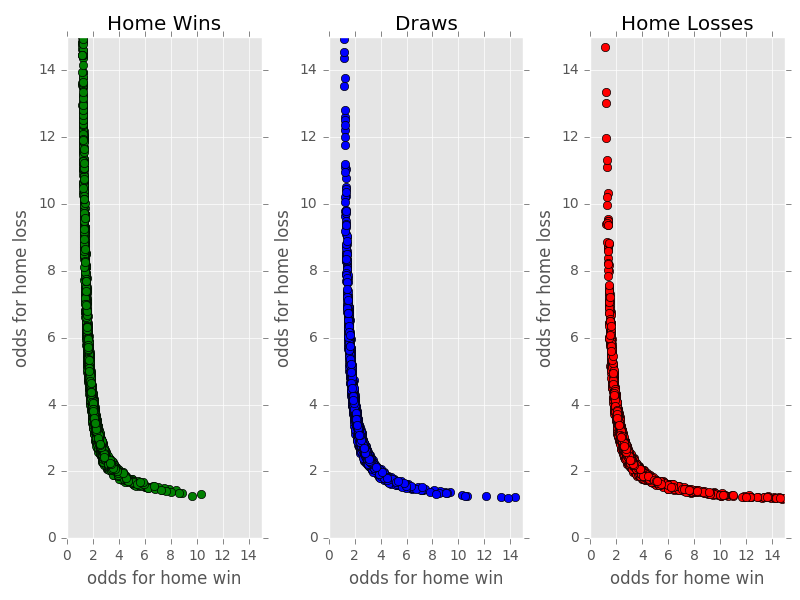
\includegraphics[width=0.8\textwidth]{2D_15.png}
		\caption{Scatter plot of data points with odds for home loss versus odds for home win. The dataset plotted is from season 2015 and beyond. A high odds for home win suggests a low odds for home loss, and vice versa.}
	\end{figure}
	
	A 3D plot of data points for all three features, $h, d$ and $a$, is as following:
	\begin{figure}[!ht]
		\centering
		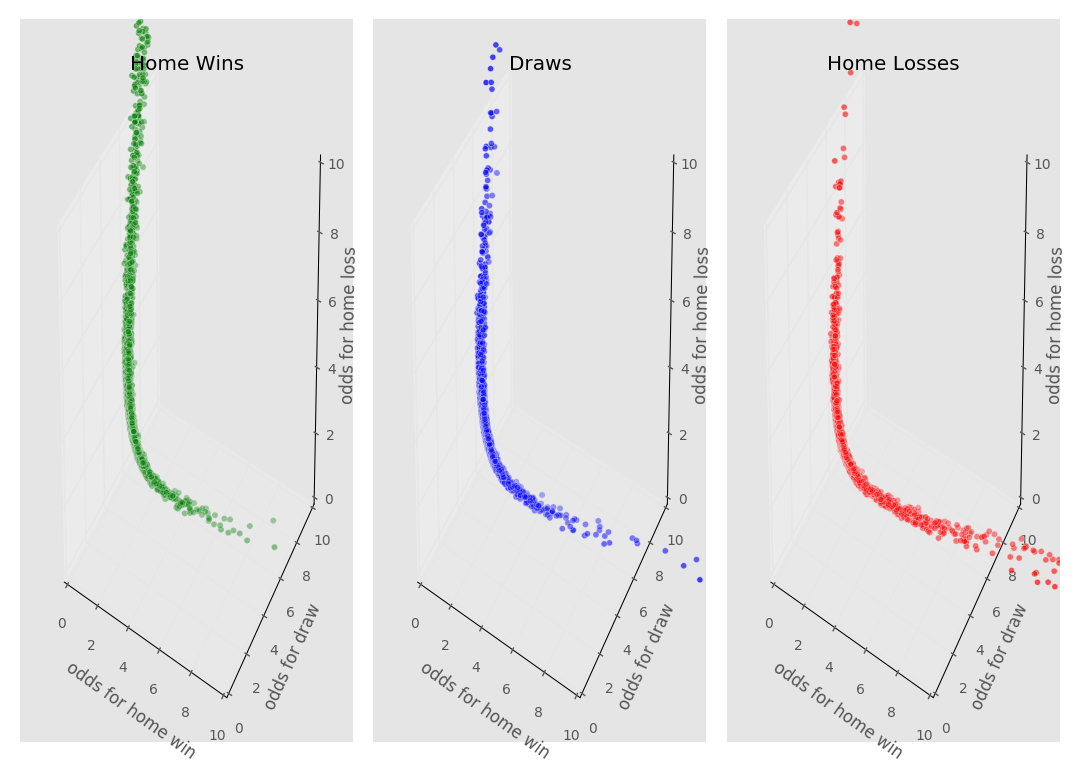
\includegraphics[width=0.8\textwidth]{3D_15.png}
		\caption{3D Scatter plot of data points with odds for all three features. The dataset plotted is from season 2015 and beyond.}
	\end{figure}
	
	Notice that for both 2D and 3D scatter plots, we have the shape of the curves similar in all class labels, while the cluster of data takes place at slightly different coordinates.
	
	\subsubsection{Adjusting Odds for a Single Company}
	\label{single_comp}
	Suppose for match $i$ we have a set of bet data $(h_i, d_i, a_i)$, where $h_i, d_i, a_i$ stand for the gambling rate for this match for home win, draw, and home loss, respectively. We want to generate a single feature that is able to characterize the three gambling odds provided. The characterization we provide here is \[
	x_i = \log(\frac{1}{3}(\frac{h_i}{a_i} + \frac{h_i}{d_i} + \frac{d_i}{a_i}))
	\]
	
	Suppose in this match we have $h_i \ll d_i \ll a_i$. This indicates that the home team is very likely to win. We have $\frac{1}{3}(\frac{h_i}{a_i} + \frac{h_i}{d_i} + \frac{d_i}{a_i}) < 1$, and hence we will have $x_i < 0$. 
	
	By symmetry, if $h_i \gg d_i \gg a_i$, the data suggests a home loss, and we will have $x_i > 0$.
	
	If $h_i \approx d_i \approx a_i$, the data suggests a high likelihood of draw, and we will have $x_i \approx 0$.
	
	Hence, the value of $x_i$ is a good indicator of the result of the match.
	\subsubsection{Adjusting Odds for Multiple Companies}
	\label{multi_comp}
	The previous section discusses the characterization of bet data for a single company. In the following section, we will discuss how to characterize the data for multiple companies.
	
	Suppose we have a list of odds for home wins from $k$ companies for a match $i$, say, $[h_{i1}, h_{i2} \ldots h_{ik}]$. We want to find the expected odds for home win from these $k$ values. Recall that $h_i$ stands for the amount of money you would receive if you bet bome win for one unit of money, given that the home team wins eventually. Suppose each bet company has an equal weight of $\frac{1}{k}$. We can see that \[
	E(h_i) = \sum_{j = 1}^{k}h_{ij}p(j) = \sum_{j = 1}^{k}h_{ij}\frac{1}{k} = \frac{\sum_{j = 1}^{k}h_{ij}}{k}
	\]
	for $k$ companies. Similarly, we have $
	E(a_i) = \frac{\sum_{j = 1}^{k}a_{ij}}{k}$ and $ E(d_i) = \frac{\sum_{j = 1}^{k}d_{ij}}{k}$.
	
	Therefore, we have our adjusted feature \[
	x_i = \log(\frac{1}{3}(\frac{E(h_i)}{E(a_i)} + \frac{E(h_i)}{E(d_i)} + \frac{E(d_i)}{E(a_i)}))
	\]
	
	
	
	\section{Algorithms}
	
	In this section, we will introduce four main algorithms to this problem, including a naive guessing algorithm, a polynomial regression algorithm, classification algorithms based on an integrated feature, and a support vector machine algorithm on multiple features. \footnote{The implementations for all algorithms discussed below is accessible at \url{https://github.com/Haunter17/BigData/tree/master/189proj}}
	
\subsection{Naive Guessing}

Intuitively, given a set of odds $(h, d, a)$ for a match, we would look for the result corresponding to the minimum value of the odds to be our prediction. In other words, the higher the gambling rate is, the more money will be awarded if the result becomes true, and the less likely the result will happen.

Based on the intuition, we make predictions on the validation dataset based on the minimum rate without training any data. The accuracy obtained is $23.78 \%$, even less than the expected value for a random guessing without knowing the odds, which is $\frac{1}{3}$.

\subsection{Polynomial Regression}
\label{poly_reg}
The first model we tried is linear regression. We use the "adjusted odds" described above as the $x$ data. Instead of using $y_i$ directly as $\mathbf{Y}$, which indicates the match result, we use the goal difference $yd_i$. The reason is that in this way the data will be more spread out instead of clustered at 1, 0 and -1. As a result our fitted curve will get a smoother and more significant slope. With this method, our prediction for validation set will also yields score difference. Thus in order to convert the score difference back to match result (denoted by 1, 0, -1), we have the following rules:
\begin{itemize}
	\item If $yd_{pred}^{(i)} > 0.5$, we predict that $\hat{y_i} = 1$, indicating a home win.
	\item If $-0.5 \leq yd_{pred}^{(i)} \leq 0.5$, we predict that $\hat{y_i} = 0$, indicating a draw.
	\item If $yd_{pred}^{(i)} < -0.5$, we predict that $\hat{y_i} = -1$, indicating a home loss.
\end{itemize}

\begin{figure}[!ht]
	\centering
	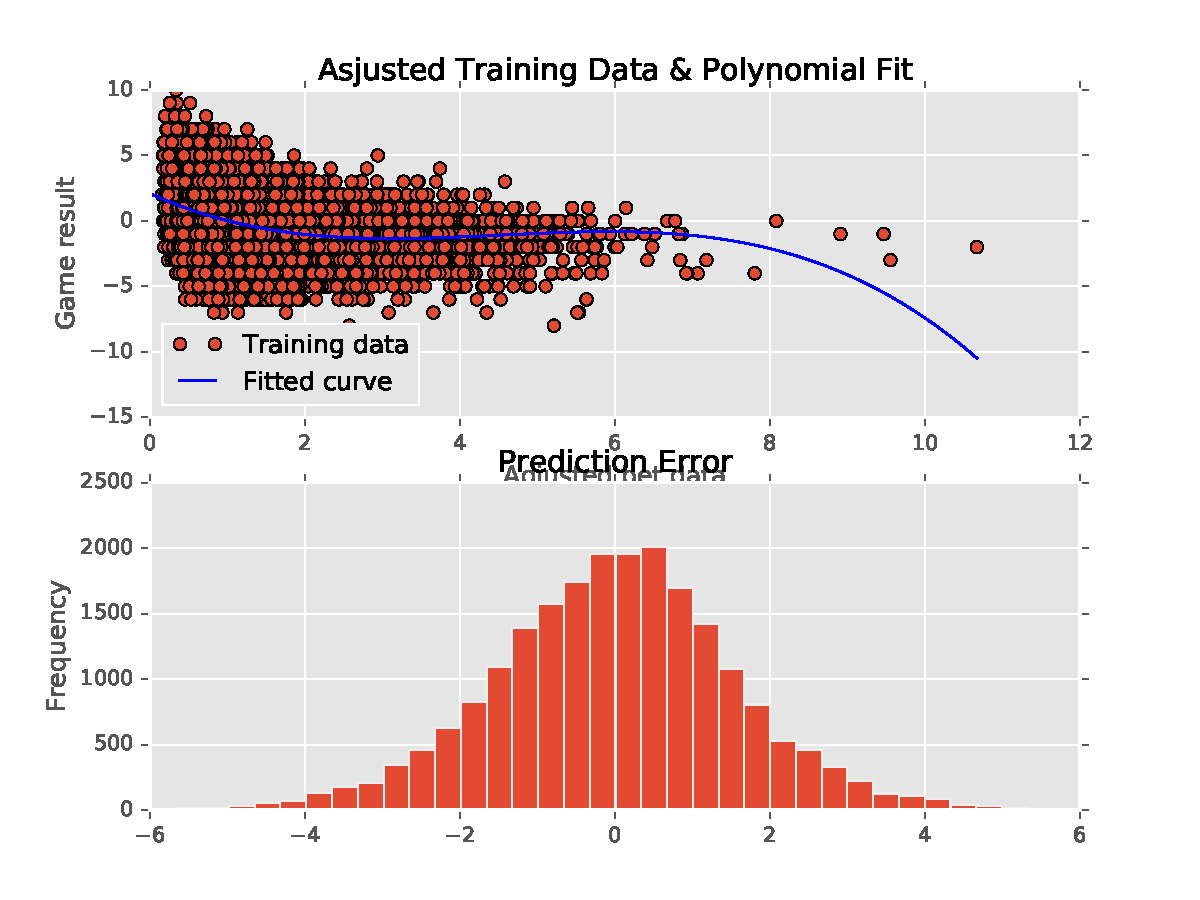
\includegraphics[width=0.5\textwidth]{linreg.png}
	\caption{Polynomial regression model fit $y = -0.048x^3 + 0.653x^2 -2.668x + 2.081$ }
	\label{fig_polyreg}
\end{figure}

Through experiment, we found that a third-order polynomial most accurately describes the data and yields the highest prediction accuracy, 0.4443. In the graph above, the top diagram shows the distribution of training data and our third-order polynomial fit. The bottom diagram shows the distribution of the prediction error using our fitted curve against the data of the validation set.



\subsection{Multi-class Classification with Single Feature}

Next, we describe a classification model using an integrated feature. This is the feature that we used for polynomial regression in Section \ref{poly_reg}, as described in Section \ref{single_comp} and Section \ref{multi_comp}. The following is a histogram showing the number of data points falls according to Figure \ref*{fig_integrated}:
\begin{figure}[!ht]
	\centering
	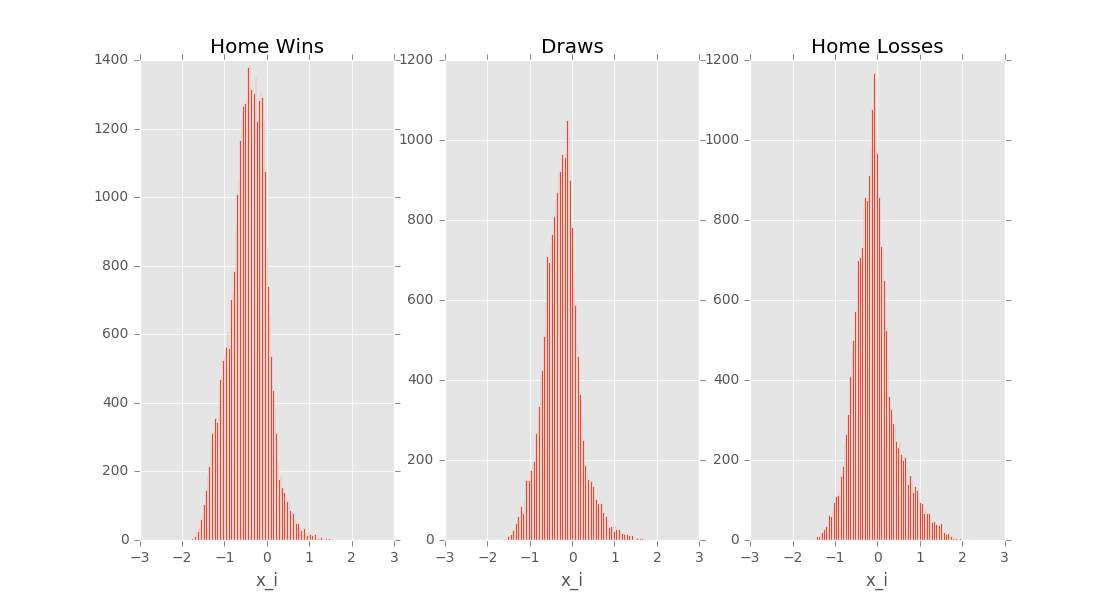
\includegraphics[width=0.8\textwidth]{1D_all.png}
	\caption{Histogram of data over the integrated feature, $x_i$.}
	\label{fig_integrated}
\end{figure}

The shape of the three subplots resembles a gaussian distribution as the datasize increases. Furthermore, the mean for each class is different, with the mean for home win to be the minimum and the mean for home loss to be the maximum.

Based on our observations above, we generate a gaussian distribution for each of the three classes with \[
\mathcal{N} (\mathbb{E}_k[x], \mathbb{V}_k[x]),
\] where $\mathbb{E}_k[x], \mathbb{V}_k[x]$ are the mean and variance of the feature $x$ in class $k$, for $k = \{-1, 0, 1\}$ corresponding to the match results.

Then, to predict the result given a set of odds for a match, we first transform the odds $(h_i, d_i, a_i)$ to get $x_i$, and we then calculate the probability density of $x_i$ in each of the three distributions. We predict \[
\hat{y_i} = \arg\max_k(p_k)
\] where $p_k$ is the probability density of class $k$, to be the distribution with the highest pdf.

We run the prediction on the validation set to predict $\hat{y_i}$ for each match, and then compare with the real result $y_i$. The prediction accuracy of the algorithm is $48.14 \%$.

We also fit the data in the model of Laplace distribution with parameters $\mu = 
\mathbb{E}_k[x]$ to be the mean and $\lambda = \sqrt{\mathbb{V}_k[x]}$ to be the standard deviation of the training dataset for each class, and we repeat the procedure above. The accuracy obtained is $47.54\%$.
\subsection{Support Vector Machine with Extended Features}

Finally we tried using Support Vector Machine, where we seek to find the optimal boundaries to differentiate between the three game outcomes using a set of features. Instead of applying the three types of input data directly, we derived 3 features based on the training data and feed them into the SVM model of $\texttt{sklearn}$ package. Note that for this model we didn't use the adjusted odds data described above. Instead, we derived the features directly from the training data for each match: $[h_i, d_i, a_i]$. The three features we use are: $h_i^2$, $\sqrt{d_i}$ and $a_i$. These features are direct variations of the training data. We increase the impact of home win while mitigate the impact of draw, since we figured that drawing bets values are somewhat inconsistent between matches. With this model we yield an accuracy of $49.17 \%$, which is so far the highest accuracy we could achieve.


\section{Discussion}
\subsection{Performance of Different Algorithms}

\subsubsection{Accuracy}
In total we tried 3 different models to analyze the betting data and make predictions about future matches. The naive guessing algorithm, based on the minimum entry of odds, does a poor job for prediction and we therefore exclude the discussion for the naive algorithm. The prediction accuracy for the other algorithms discussed are listed in \ref{sample-table}:

	\begin{table}[t]
		\caption{Prediction accuracy of different algorithms}
		\label{sample-table}
		\centering
		\begin{tabular}{ll}
			\toprule
			\multicolumn{2}{c}{Table}                   \\
			\cmidrule{1-2}
			Algorithm     & Prediction Accuracy    \\
			\midrule
		Polynomial Regression & 44.43 \% \\ 
		Classification with Integrated Feature (Gaussian) & 48.14 \% \\
		Classification with Integrated Feature (Laplace) & 47.54 \% \\
		Support Vector Machine & 49.17 \% \\
			\bottomrule
		\end{tabular}
	\end{table}

From the table, we can see that the support vector machine algorithm has the best prediction accuracy, being slightly higher than the classification algorithms with a single integrated feature. These classification algorithms has a better prediction rates than the polynomial regression algorithms.

In terms of applicability, the two classification models are better than the regression model. The main reason is that no matter we use match results or goal differences, the $\mathbf{Y}$ data is discrete. Therefore regression is not very desirable. Figure 1 reveals that the standard deviation of training data relative to the fitted curve is relatively large, so the curve does not fully represent the distribution of the data. The two classification models, on the other hand, are more appropriate in the discrete case.

\subsubsection{Running Time Efficiency}
In terms of running time efficiency, the classification algorithms with a single integrated feature runs much faster than other algorithms, while support vector machine, despite being the optimal with respect to prediction accuracy, has the longest running time. Running basic benchmark on a 2.9 GHz Intel Quad-core machine with 16 GB memory and OSX Sierra, the regression model takes about 0.03 seconds to complete and the multi-class model takes about 5 seconds to generate the prediction. To the contrary, the SVM model takes about 3 minutes to complete. Thus, the regression model and multi-class classification models are more desired in terms of performance.

\subsection{Next Steps}
\subsubsection{Possibly Optimal Algorithms}

From the figure of 2D scatter plot in Section \ref{2d_figure}, we can see a trend of one feature increasing as the other feature decreases, and vice versa. Also, observe that the cluster of the three classes are slightly different with each other.

One potential algorithm is to first find a fitting curve according to the scattered data points, and then generate a distribution for each class according to the data cluster for each class. The probability density contour of the distribution aligh roughly along the curve. Then, given a set of odds $\hat{x} = (h, a)$, we predict the probability density of $\hat{x}$ for each of the three distributions, and take the class label corresponding to the highest probability to be the prediction.

\subsubsection{Better Training Assumptions}

In this experiment, we treat all the matches equally in terms of the background of the matches. However, there might be underlying features that affect the accuracy of the prediction. For instance, we can add a feature representing the competitiveness of the league, giving different weight between top level leagues and low level leagues. Furthermore, we can take the country of the league into account as well. With these extended features, the data might become more separable and the fitting algorithms are likely to have better performance.

\section*{Acknowledgments}

We received help on algorithm design from Professor Weiqing Gu, Professor Robert Keller, and Natchanon Suaysom, one of the teaching assisstants.

\section*{References}

	\medskip
	
	\small
	
	[1] Murphy, Kevin P.\ (2012)  {\it Machine learning: a probablistic perspective}. Cambridge, MA: MIT Press.
	
\end{document}